\section{Introduction}
\label{sec:introduction}

In the literature, video understanding tasks, 
such as action recognition~\citep{activitynet,something,kinetics}, 
visual object tracking~\citep{got_10k,trackingnet}, 
and video question-answering~\citep{msrvtt_qa,jang2017tgifqa,next_qa,li2024mvbench}, 
have primarily focused on short clips lasting from a few seconds to minutes. 
However, as vision models increasingly find applications in real-world scenarios like robotics, surveillance, and live broadcasts, the research in the vision community has gradually shifted towards understanding continuous video streams, where long-term contexts and real-time interaction are crucial.

In this paper, we consider the problem of \textbf{streaming video question-answering (StreamingVQA)}. As shown in Figure~\ref{fig:teaser}(a),
it involves continuously processing long video streams and promptly responding to queries about the visual content at any moment. It can be treated as a generalization of the standard offline VideoQA, where the model processes the entire video and all questions simultaneously. By definition, such task of StreamingVQA presents three core challenges: 
(i) \textbf{Efficient Video Encoding:}
Unlike traditional offline VideoQA, where models have access to the entire video clip, StreamingVQA demands real-time analysis of continuous streams. Models must efficiently process incoming frames without access to future frames or frequent revisiting of distant past frames. (ii) \textbf{Video Context Preservation:} 
To accurately answer questions posed later in the stream, models must preserve relevant information from earlier frames, making long-term context retention a key challenge. 
(iii) \textbf{Real-Time Response:} 
The model must provide accurate answers with minimal delay, requiring efficient retrieval of video context and rapid question-answering.

Current Video-LLMs often struggle to encode long video streams due to the large volume of video tokens, forcing most models to process only a sparse subset of frames~\citep{video_chatgpt, llava_next_video, llava_onevision}. 
This results in limited video lengths or a significant loss of fine-grained visual information. While techniques like average pooling~\citep{llamavid} and memory compression~\citep{wu2022memvit,wang2023memory,he2024ma,flashvstream,videostreaming} reduce token volume, they come at the cost of losing details, particularly in temporal and lower-level visual features that are essential for complex question answering.

% 为了方便修改,我们可以先定义一个统一的高度变量
\newlength{\myfigheight}
\setlength{\myfigheight}{7.01cm} % 在这里统一调整三张图的高度

\begin{figure*}[t]
    \centering
    
    % --- 子图 (a) ---
    \begin{subfigure}{\widthof{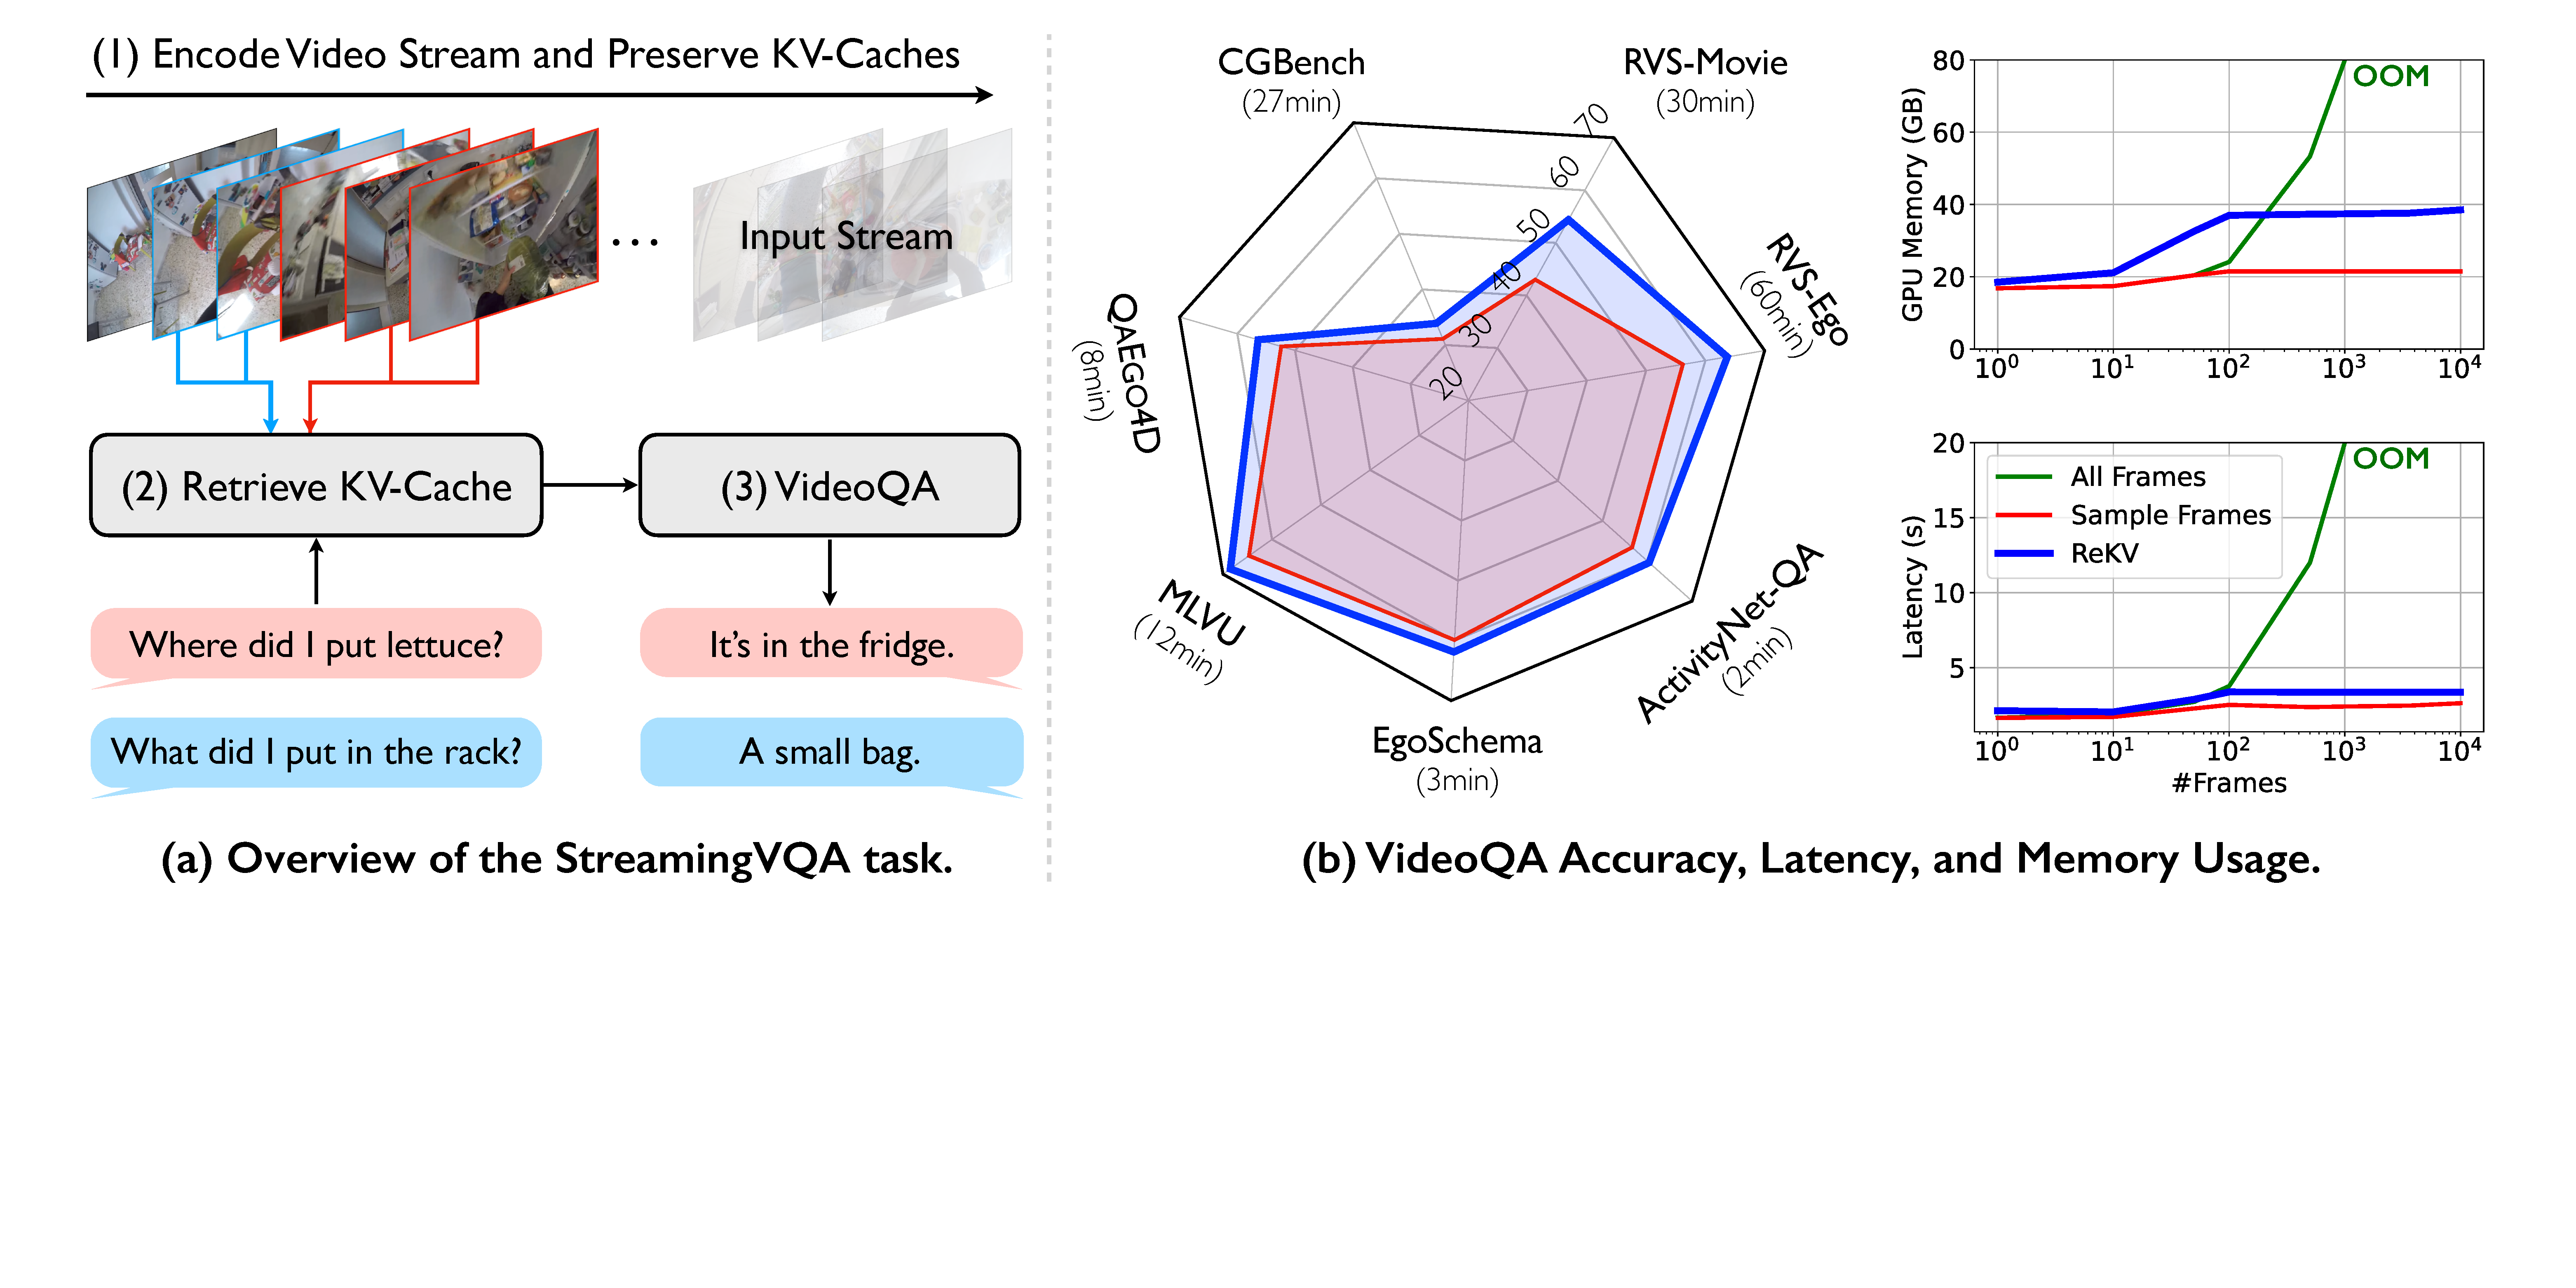
\includegraphics[height=\myfigheight, trim={0 0 415pt 0}, clip]{figures/teaser.pdf}}}
        \centering
        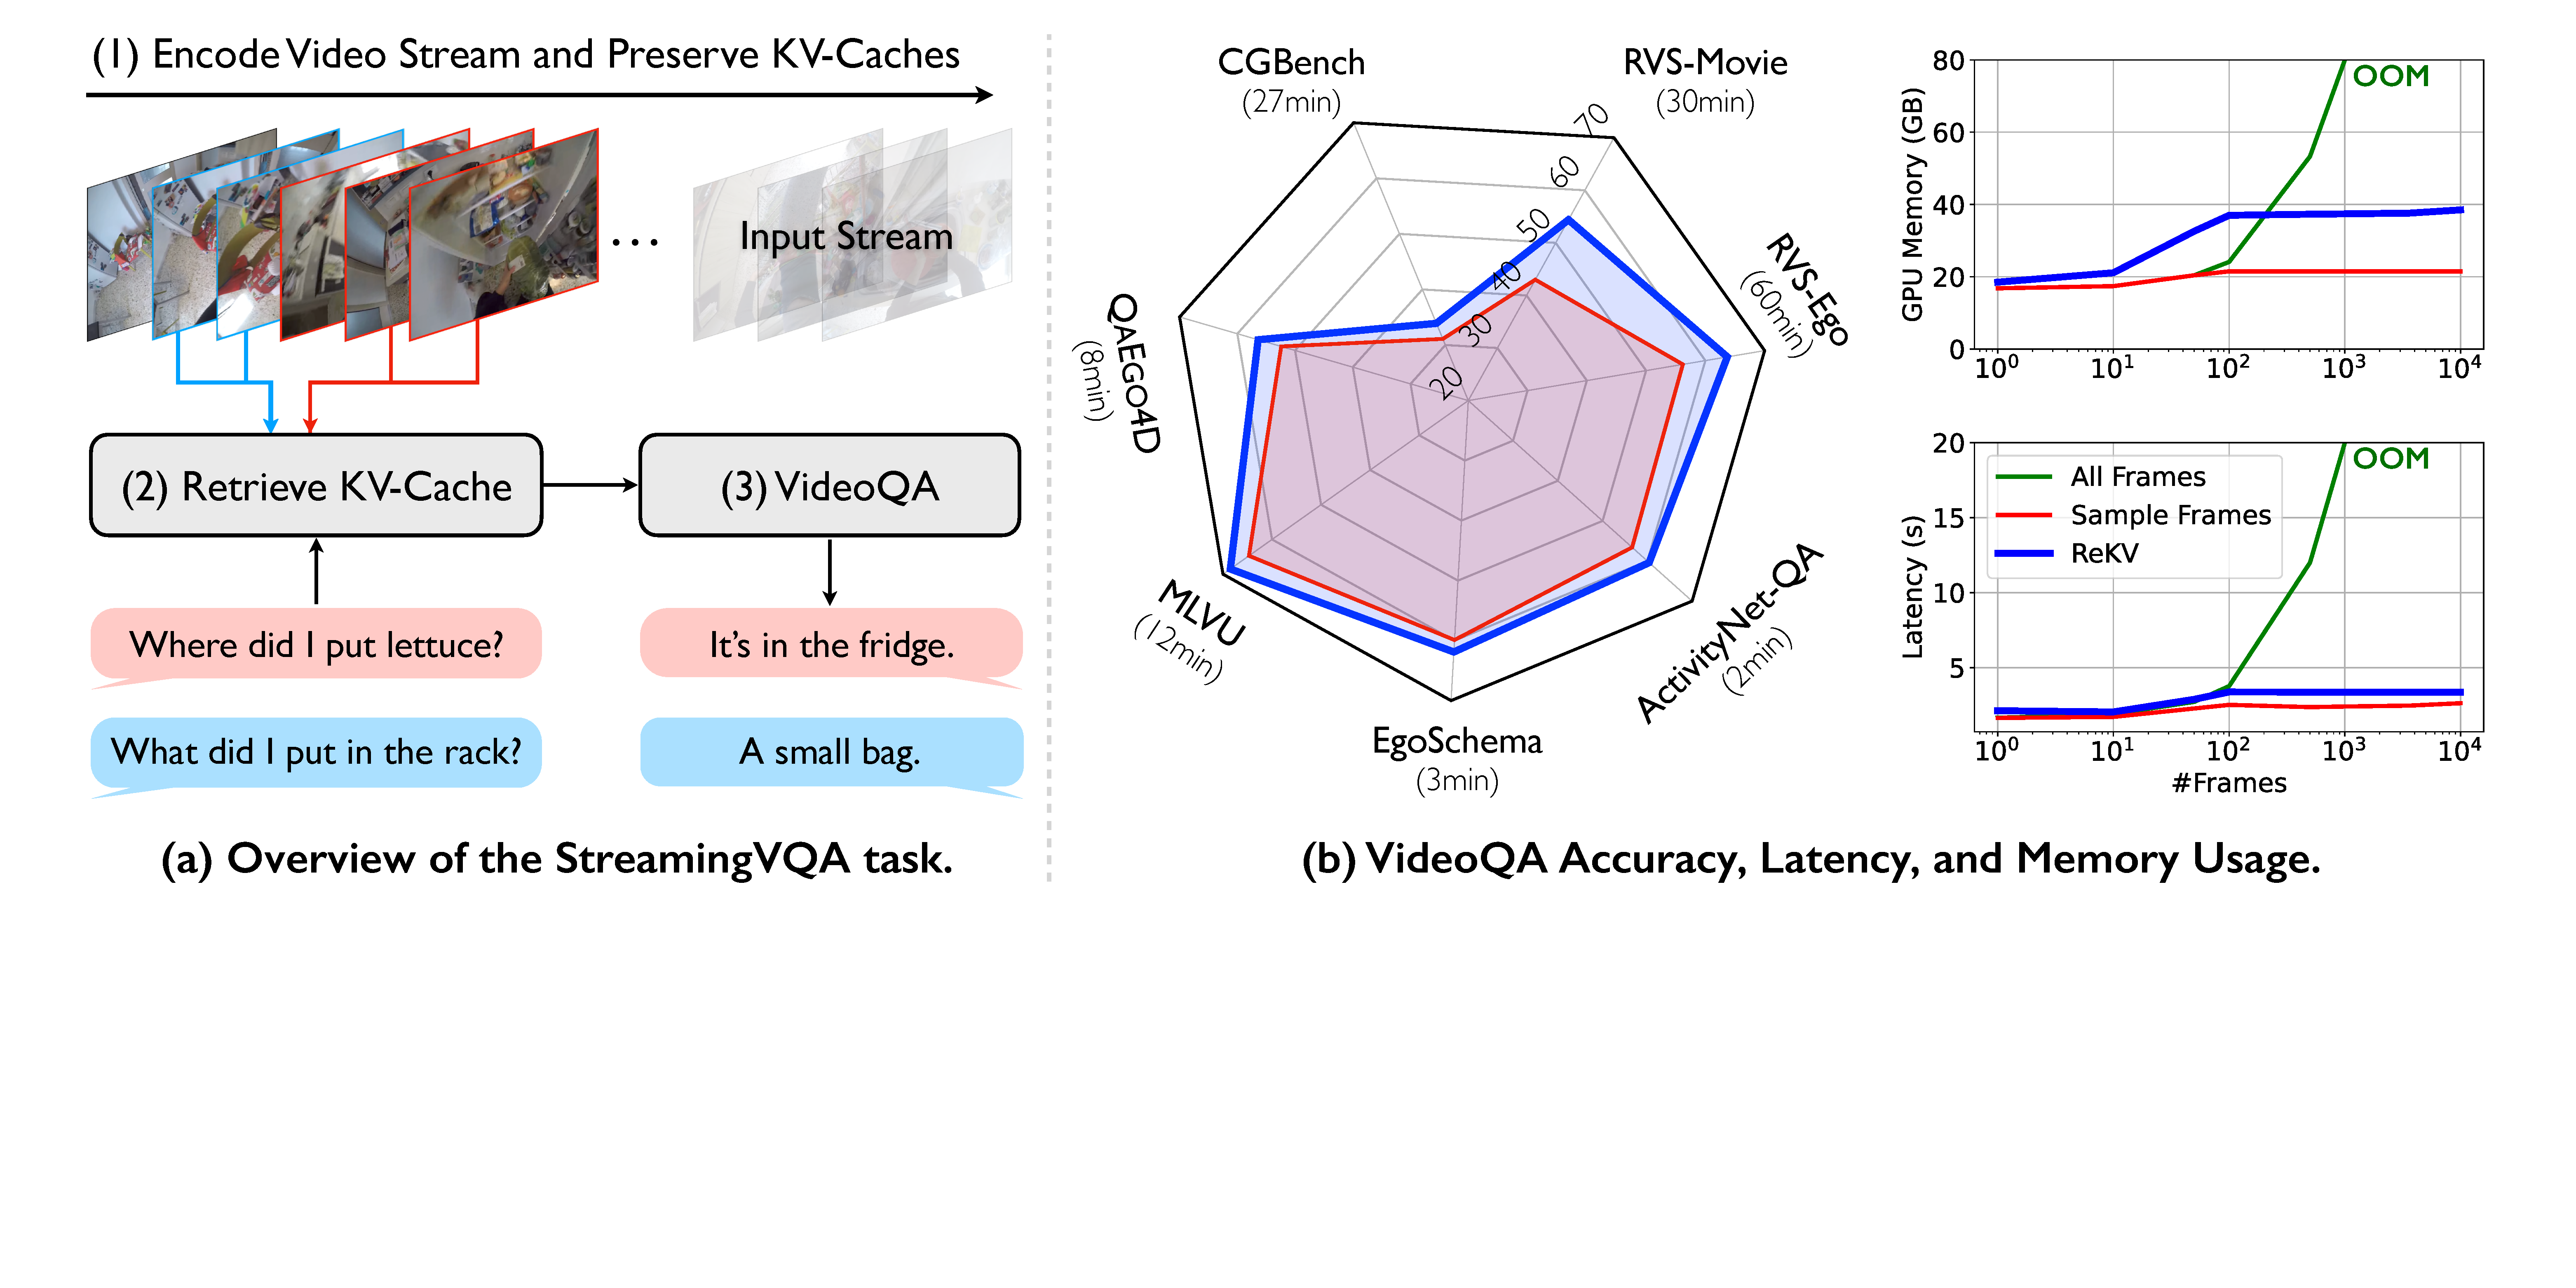
\includegraphics[height=\myfigheight, trim={0 0 415pt 0}, clip]{figures/teaser.pdf}
        \caption{\hermes Framework}
        \label{fig:teaser_a}
    \end{subfigure}
    % --- 子图 (b) ---
    \begin{subfigure}{\widthof{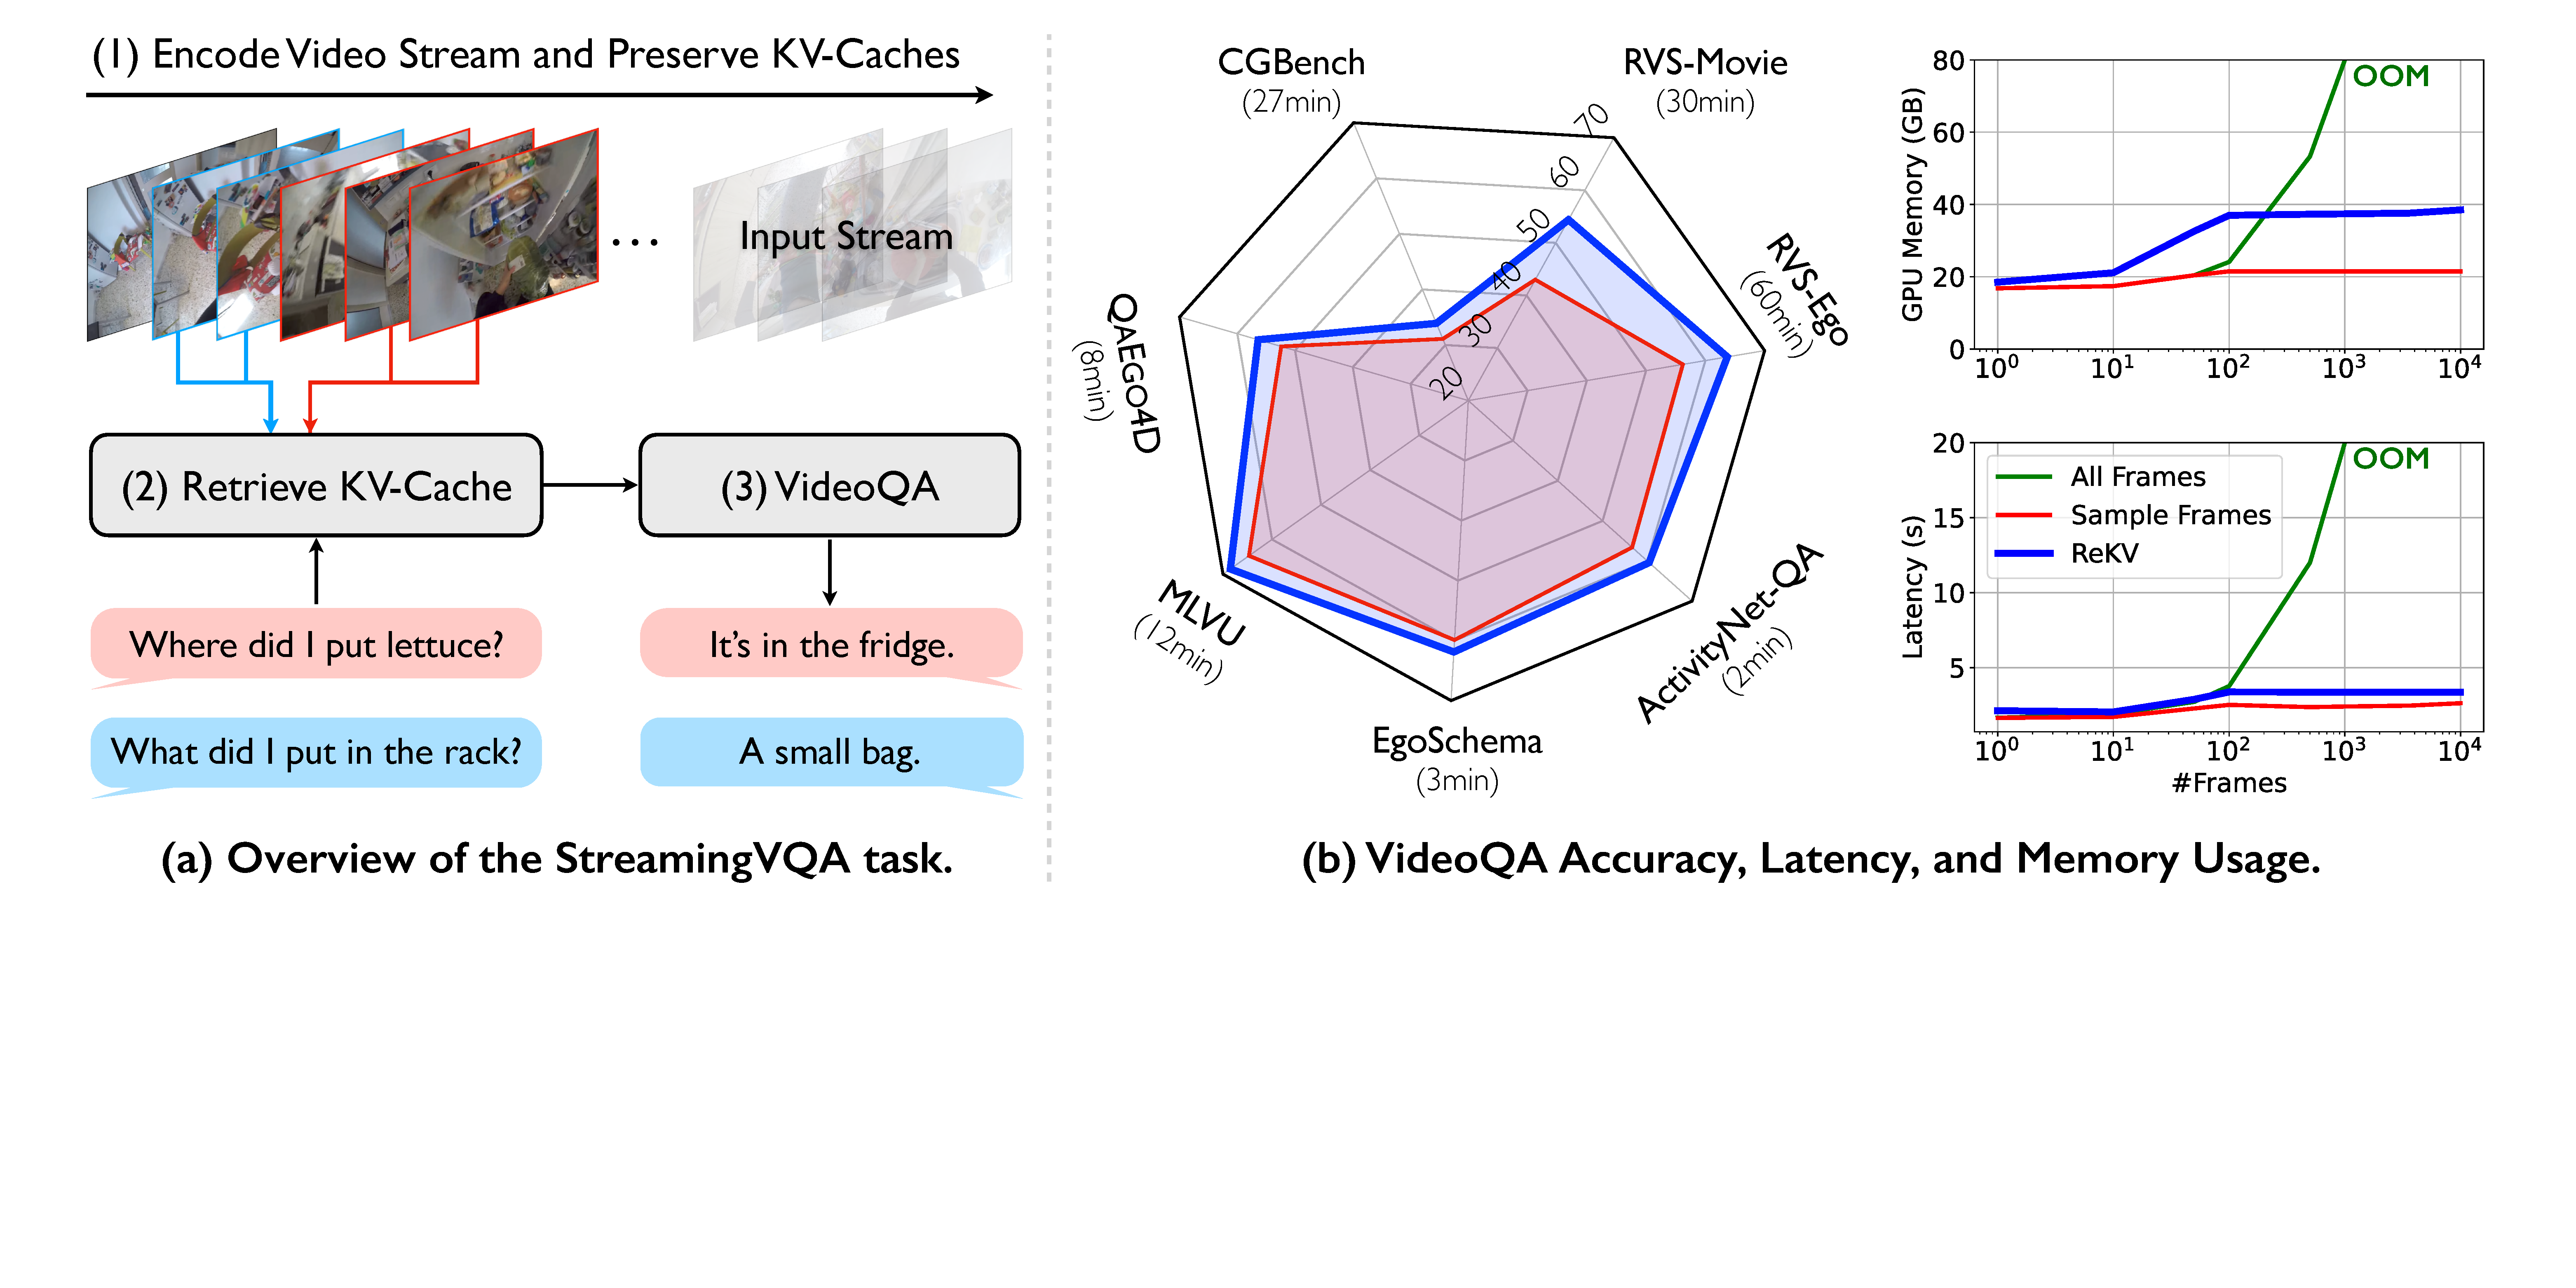
\includegraphics[height=\myfigheight, trim={365pt 0 251pt 0}, clip]{figures/teaser.pdf}}}
        \centering
        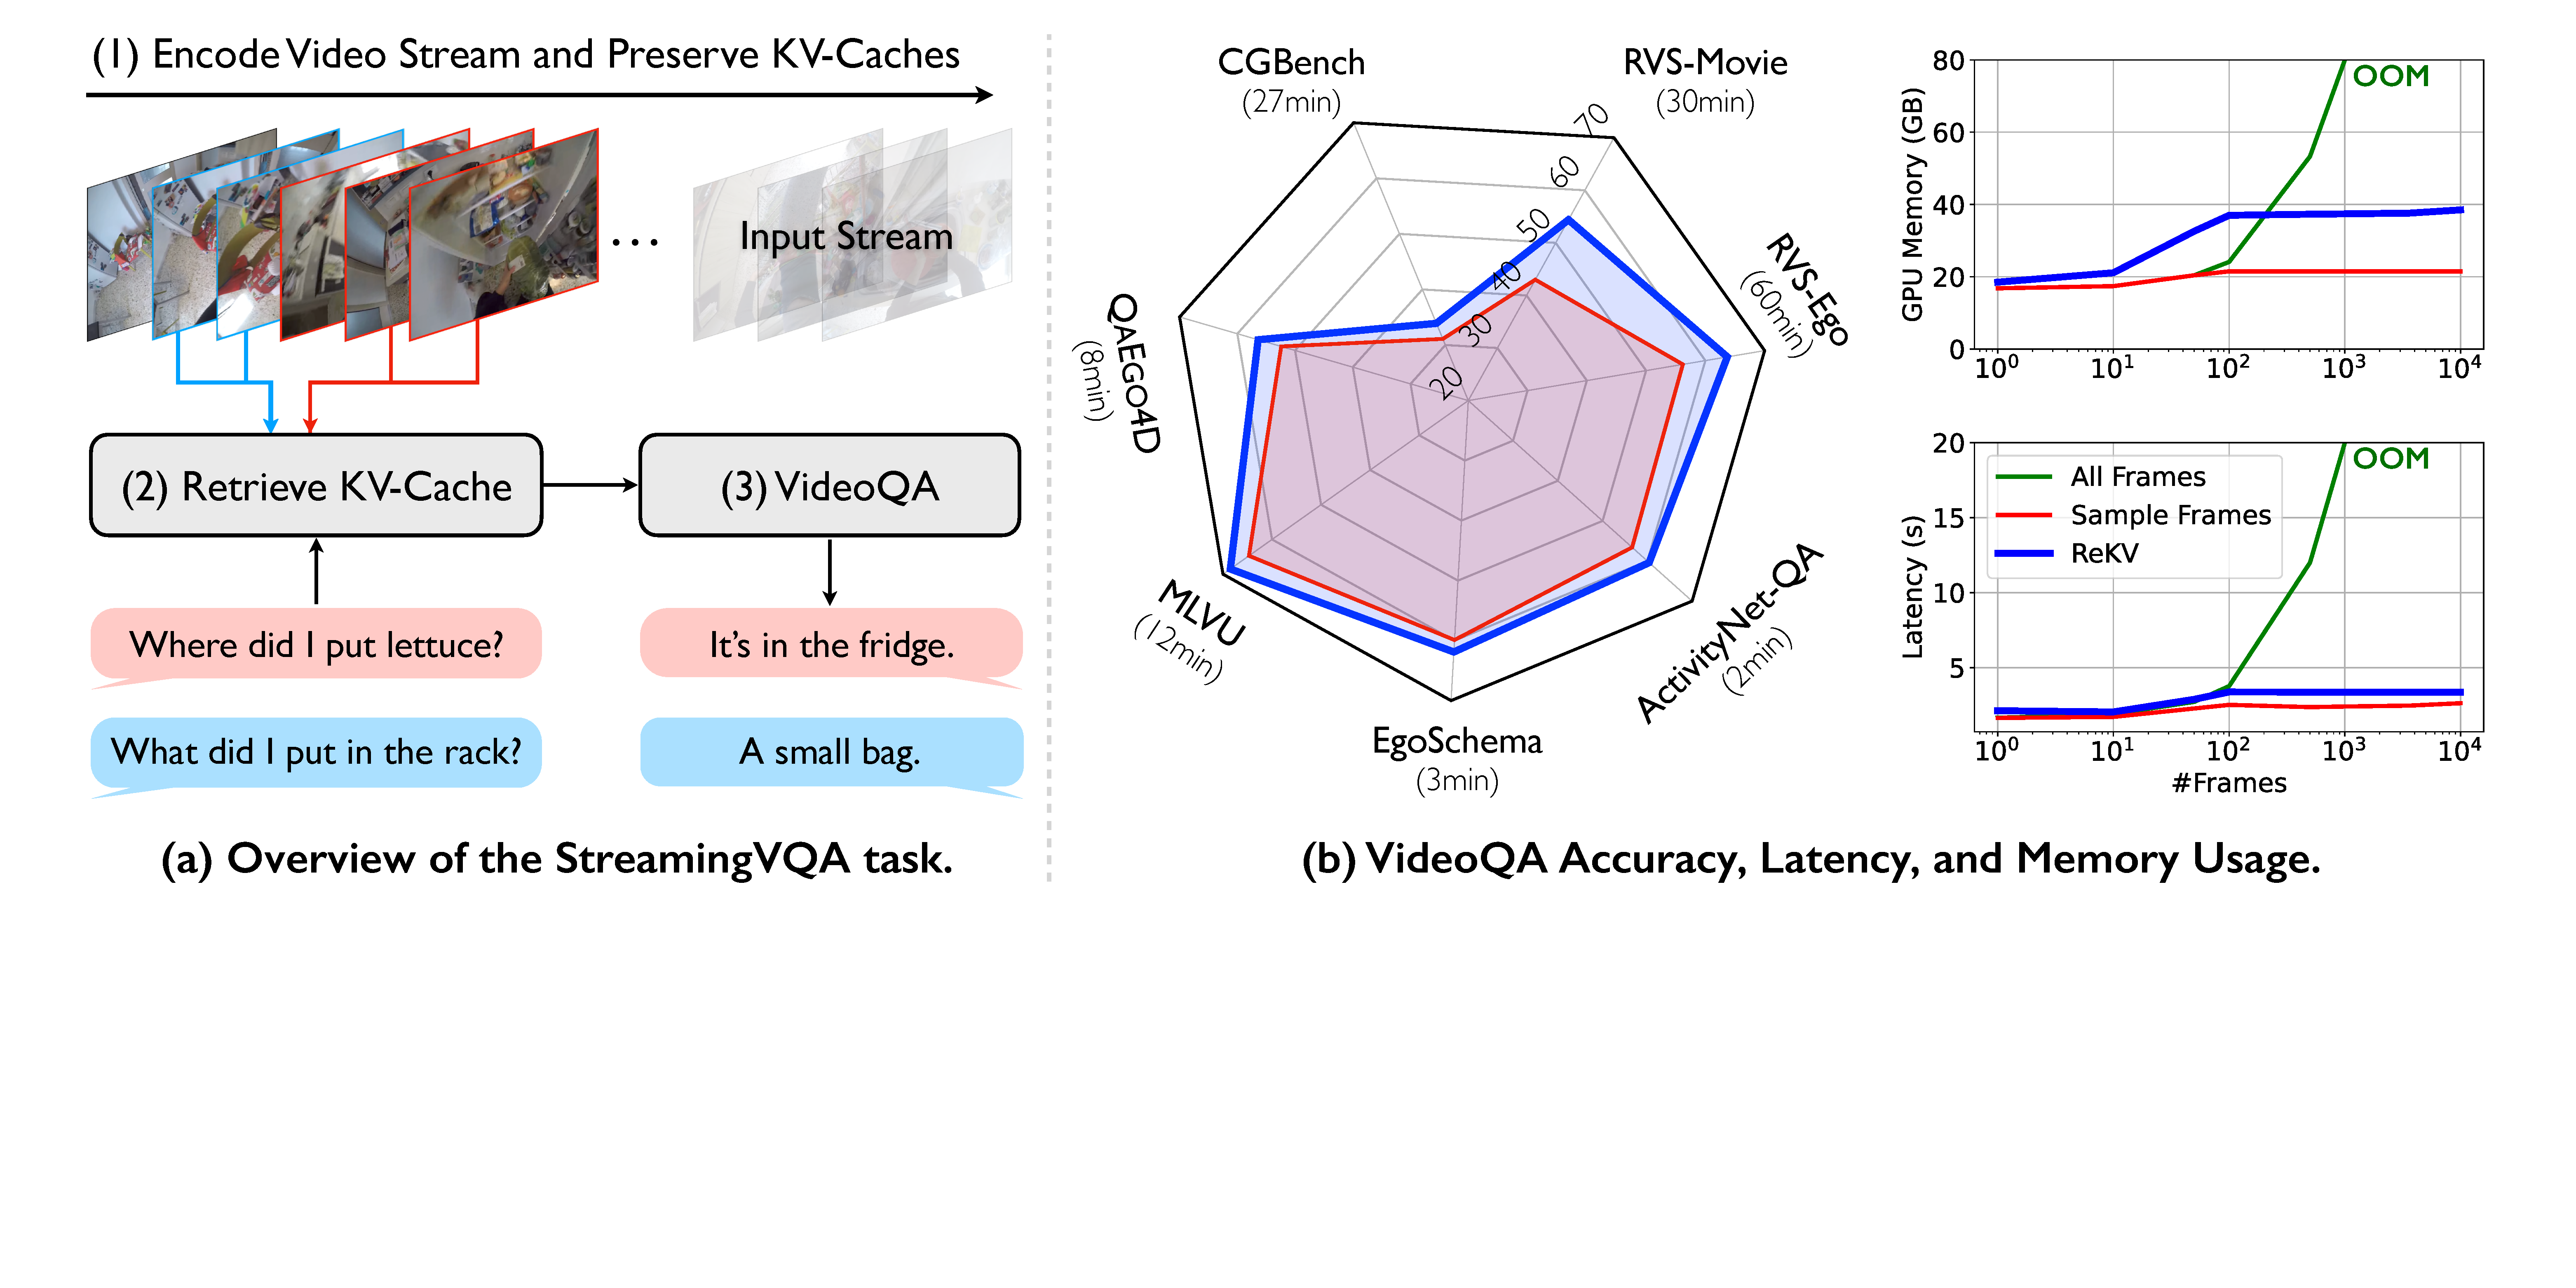
\includegraphics[height=\myfigheight, trim={365pt 0 251pt 0}, clip]{figures/teaser.pdf}
        \caption{Attention Analysis}
        \label{fig:teaser_b}
    \end{subfigure}
    % --- 子图 (c) ---
    \begin{subfigure}{\widthof{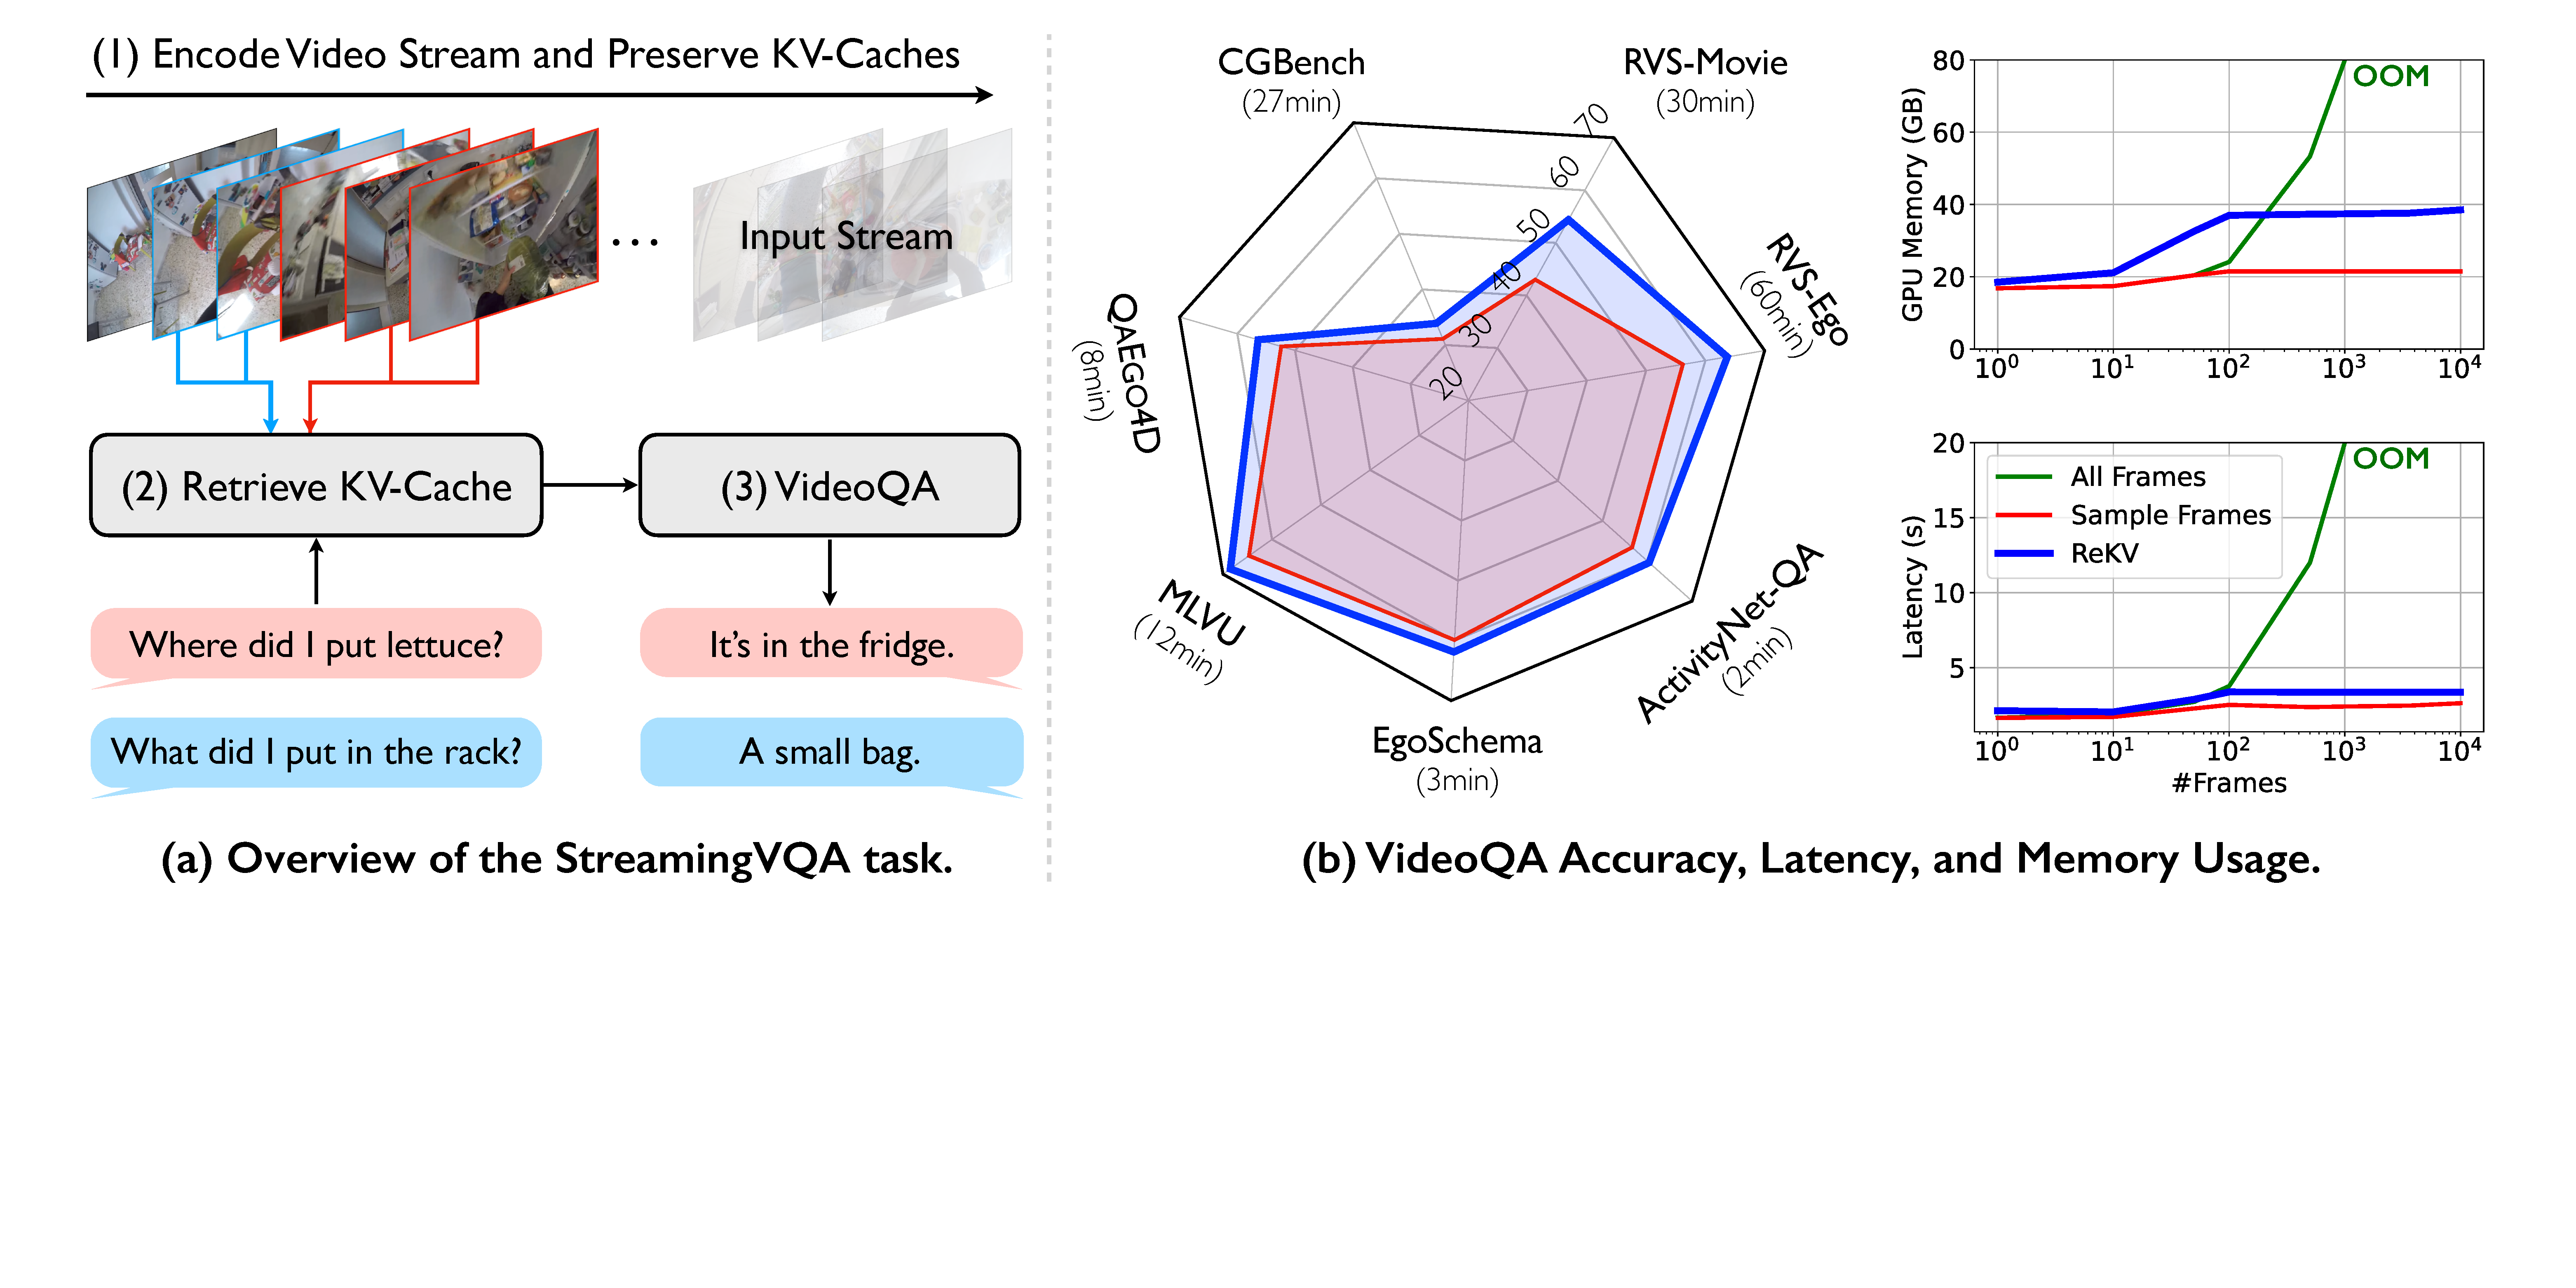
\includegraphics[height=\myfigheight, trim={529pt 0 0 0}, clip]{figures/teaser.pdf}}}
        \centering
        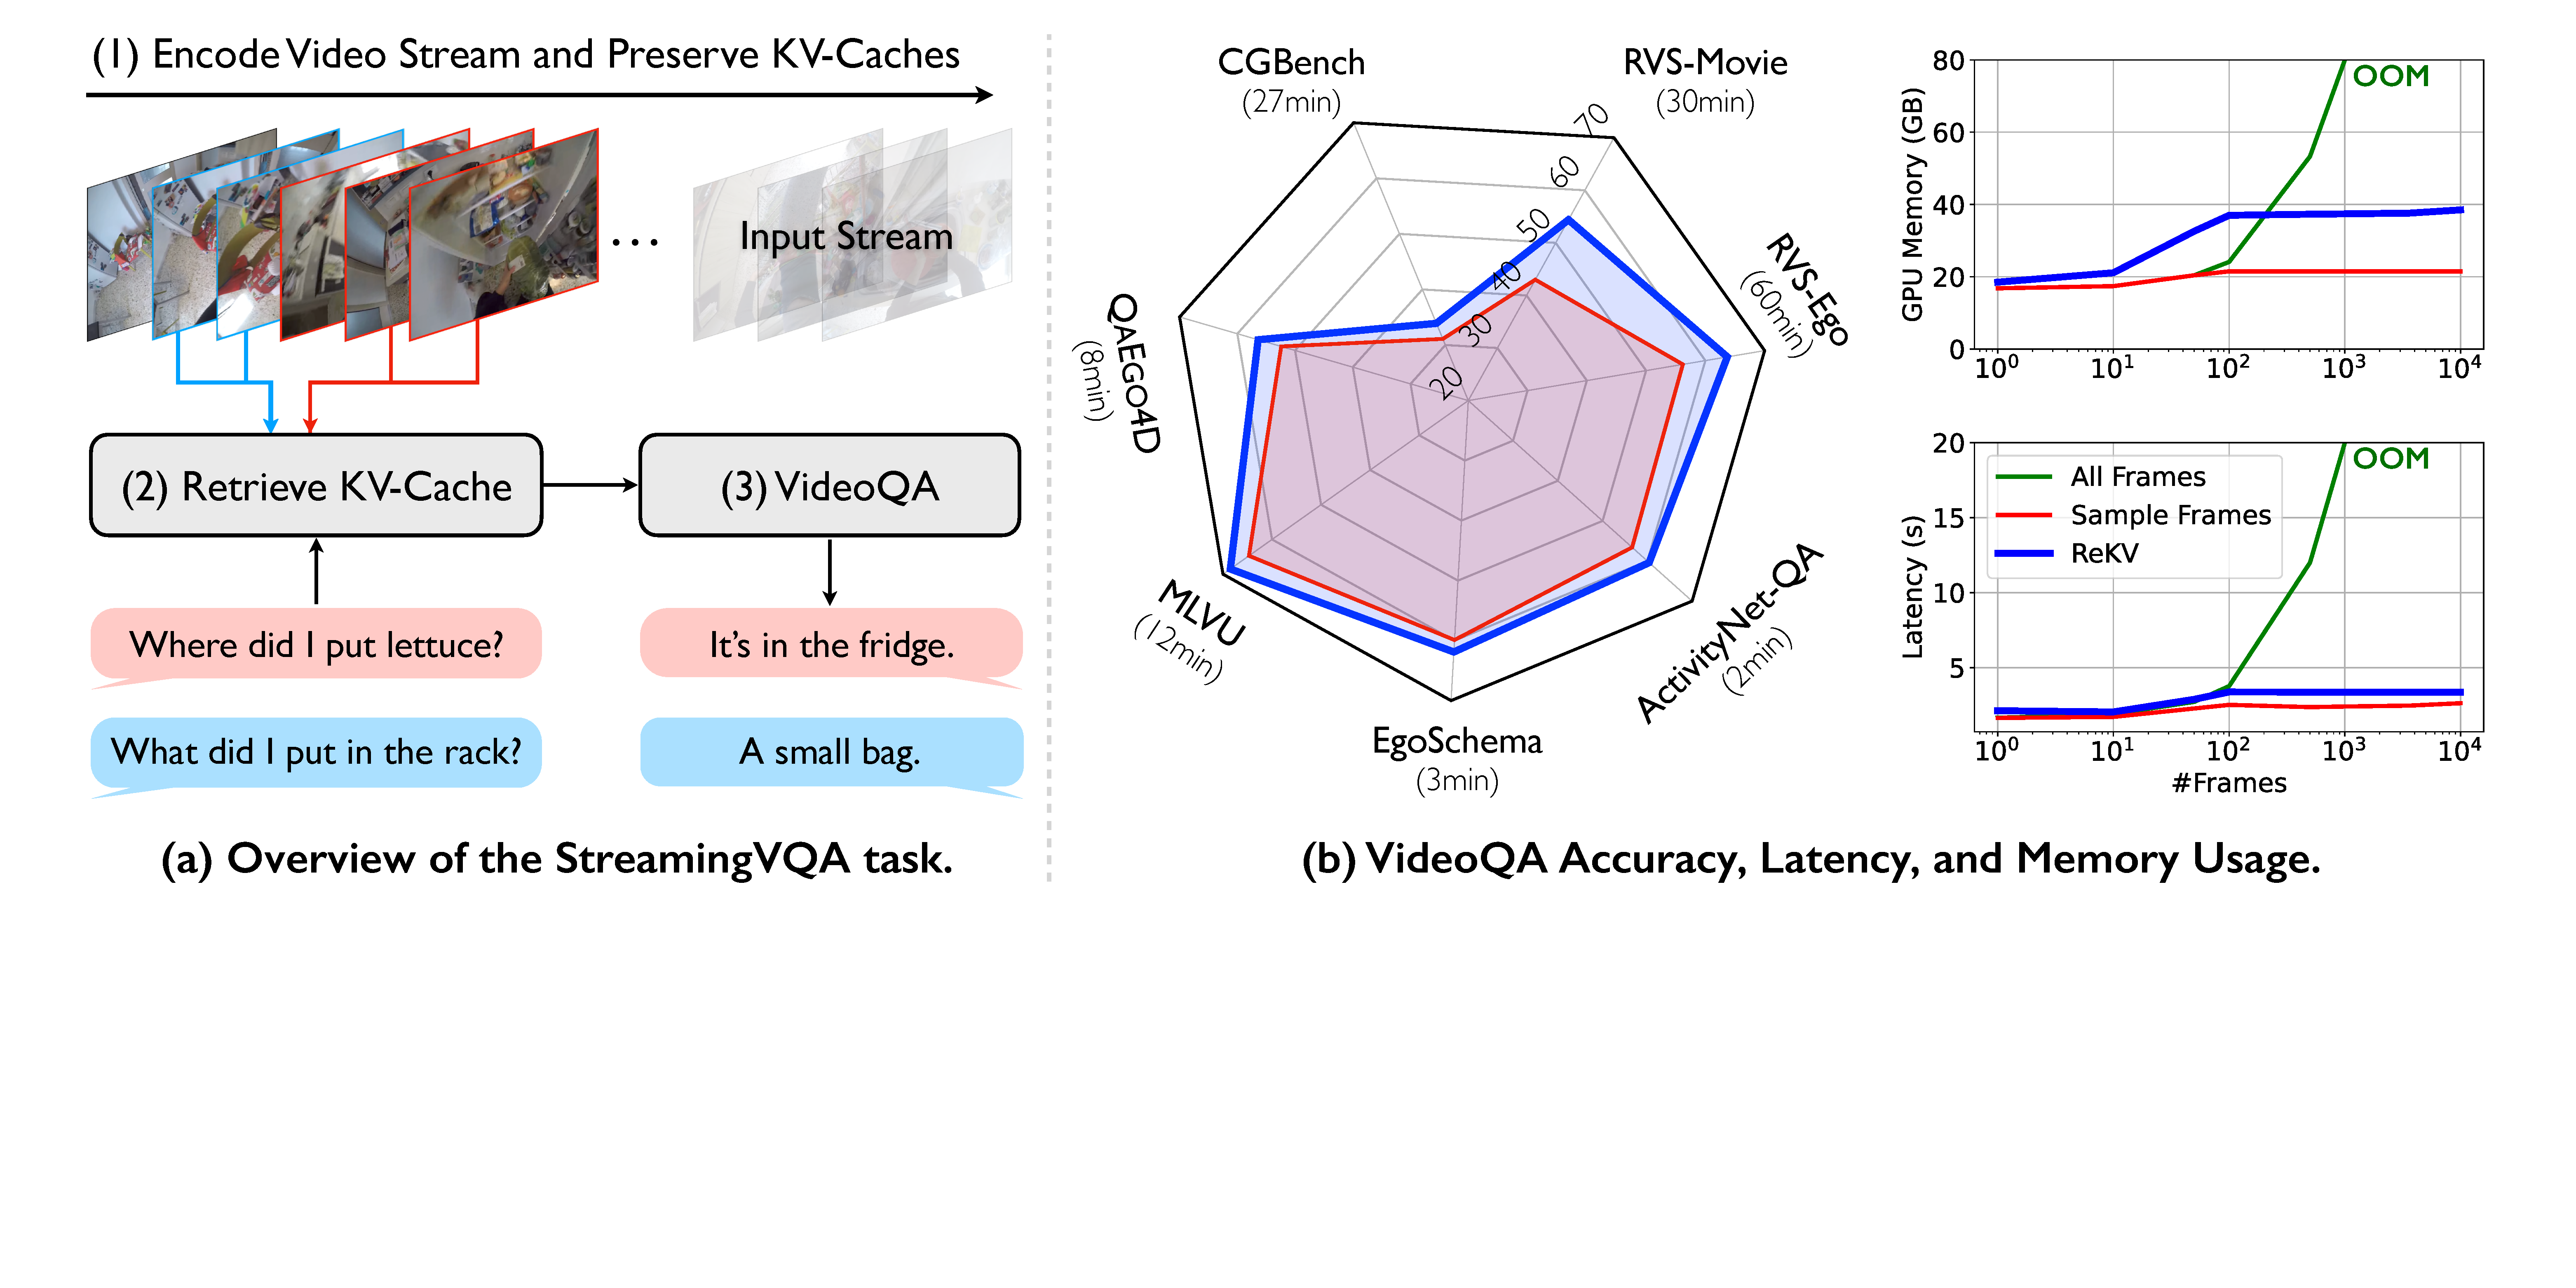
\includegraphics[height=\myfigheight, trim={529pt 0 0 0}, clip]{figures/teaser.pdf}
        \caption{Efficiency Test}
        \label{fig:teaser_c}
    \end{subfigure}
    \caption{\textbf{Left}: \hermes is a training-free approach for efficient streaming video understanding, enabling stable inference by reusing KV cache and performing hierarchical management of video tokens stored in KV cache. \textbf{Middle}: \hermes is based on a mechanistic investigation of the layer-wise attention preferences over hierarchical video information. \textbf{Right}: We evaluate \llava on a single A800 GPU (80 GB). As input frames increase, \hermes consistently maintains extremely low latency (TTFT < 30 ms) and stable GPU memory consumption, exhibiting no risk of OOM errors and requiring no auxiliary external computational resources.}
\end{figure*}




To address the challenges, we propose \textbf{\ourmethod} (\textbf{Re}trieve In-context Video \textbf{KV}-Cache), a framework that seamlessly integrates with existing Video-LLMs~\citep{video_chatgpt, llava_next_video, llava_onevision} without additional training. 
Our method employs two strategies for aggregating both short- and long-term temporal information. 
For \textbf{short-term temporal context}, 
the model adopts causal attention with a sliding-window mechanism~\citep{lm_infinite}, where tokens attend only to a limited set of preceding tokens during encoding.  
For \textbf{recalling long-term information}, 
we enable dynamic access to any point within the video sequence via retrieval. 
Specifically, our method retains and reuses past computations (KV-Cache) to avoid redundant processing while enhancing long-term reasoning without sacrificing detail. For extremely long videos, KV-Caches can be offloaded to RAM or disk to prevent memory overflow.

To ensure real-time and accurate responses, we retrieve a fixed number of KV-Caches relevant to the current question. This design strikes a balance between efficiency and accuracy by avoiding the need to process all past frames, while still accessing the most critical information. We experimented with two retrieval methods: one using external CLIP-like models~\citep{clip, siglip} for semantic matching, and another leveraging internal attention weights for faster, more integrated, and potentially stronger retrieval~\citep{infllm, snapkv}.

In summary, {\ourmethod}~efficiently encodes long video streams, 
preserves and retrieves in-context KV-Caches to address complex video question-answering. In addition, {\ourmethod}~separates video encoding from question-answering into distinct processes, further enhancing efficiency. As shown in Figure~\ref{fig:teaser}(b), {\ourmethod}~improves VideoQA accuracy while maintaining stable inference latency and memory usage as frames increase. 
The remainder of the paper is organized as follows: 
Section~\ref{sec:related_work} provides an overview of the relevant literature. 
Section~\ref{sec:method} formulates the StreamingVQA task and describes our proposed method in detail. In Section~\ref{sec:experiments}, we present ablation studies and comparisons to validate our approach. Consequently, our approach not only enhances accuracy on long VideoQA benchmarks, including MLVU~\citep{mlvu}, \textsc{QAEgo4D$_\texttt{MC}$}~\citep{di2023groundvqa}, EgoSchema~\citep{egoschema}, and ActivityNet-QA~\citep{activitynet_qa}, as well as StreamingVQA benchmarks~\citep{flashvstream}, but also reduces inference latency and memory usage. 
